% ---------------------------------------------------------
% CoreASM-UserManual.tex 	$Revision: #27 $
%
% "CoreASM User Manual"
%
% Copyright (c) 2005 Roozbeh Farahbod
%
% This work is licensed under the Creative Commons 
% Attribution-NonCommercial-NoDerivs License. To view 
% a copy of this license, visit the following link:
%
%   http://creativecommons.org/licenses/by-nc-nd/2.0/ca/ 
% 
% ---------------------------------------------------------

\documentclass{article}

\usepackage{amsmath}

\DeclareFontShape{OT1}{cmtt}{bx}{n}{
  <5><6><7><8><9><10><10.95><12><14.4><17.28><20.74><24.88>cmttb10}{}

\newcommand{\version}{First Draft: \today}%{0.9 Beta}

%\setlength{\voffset}{0in}
%\setlength{\topmargin}{-0.25in}
%\setlength{\headheight}{0.22in}
%\setlength{\headsep}{0.2in}
%\setlength{\hoffset}{0in}
%\addtolength{\textheight}{1.4in}
%\setlength{\footskip}{0.15in}
%\addtolength{\oddsidemargin}{-0.04\textwidth}
%\addtolength{\textwidth}{0.08\textwidth}
%\addtolength{\topmargin}{-0.04\textheight}
%\addtolength{\textheight}{0.08\textheight}

\usepackage{graphicx}
\usepackage{color}
\usepackage{amsfonts}
\usepackage{amssymb}
\usepackage{xspace}
\usepackage{url}
\usepackage{stmaryrd}
\usepackage{fancyhdr}
\usepackage{float}
\usepackage{makeidx}
\usepackage{psboxit} 
\usepackage{moreverb}

\usepackage[small,normal,bf,up]{caption}
\renewcommand{\captionfont}{\small}

\usepackage{float}
\floatstyle{ruled}
\newfloat{program}{thp}{lop}
\floatname{program}{Program}


\setlength{\oddsidemargin}{0.2in}
\setlength{\textwidth}{5.9in}
\addtolength{\parskip}{0.07in}

% ----------------- CoreASM Spec Float
\floatstyle{boxed}
\newfloat{coreasm}{thp}{los}[section]
\floatname{coreasm}{CoreASM Spec}
\floatstyle{plain}

\makeatletter
\newcommand\jcodename{Code}
\newcounter{jcode}
\renewcommand\thejcode{\@arabic\c@jcode}
\def\fps@jcode{btp}
\def\ftype@jcode{3}
\def\ext@jcode{lop}
\def\fnum@jcode{\jcodename~\thejcode}
\newenvironment{jcode}
               {\@float{jcode}}
               {\end@float}
\newenvironment{jcode*}
               {\@dblfloat{jcode}}
               {\end@dblfloat}
\makeatother

\makeindex
\begin{document}


\pagestyle{fancy}
%\renewcommand{\chaptermark}[1]{
%	\markboth{\thechapter.\ #1}{}}
\lhead{{\small \leftmark}}
\rhead{{\small {\scshape How to Write a \CoreASM\ plug-in}}}
% You need to turn the 'twoside' option on, 
% before uncommenting the following lines.
%\fancyhead{}
%\fancyhead[LO,RE]{{\small \leftmark}}
%\fancyhead[RO,LE]{{\small \CoreASM Execution Engine}}



% ----------------- Commands
% ---------------------------------------------------------
% asmcommands.tex	2.0 	19-Aug-2005 
%
% A series of LaTeX commands defined for 
% typesetting ASM specifications
%
% Copyright (c) 2005 Uwe Glaesser
% Copyright (c) 2005 Roozbeh Farahbod
% Copyright (c) 2005 Mona Vajihollahi
% Copyright (c) 2005 Vincenzo Gervasi
% Copyright (c) 2005 Mashaal Memon
%
% This work is licensed under the Creative Commons 
% Attribution-NonCommercial-NoDerivs License. To view 
% a copy of this license, visit the following link:
%
%   http://creativecommons.org/licenses/by-nc-nd/2.0/ca/ 
% 
% ---------------------------------------------------------

% ----------------- ASM Rule Environments
\newcommand{\bmRule}{ \noindent \small $ \begin{array}{l} }
\newcommand{\emRule}{ \end{array} $  \normalsize }

% ASM rule block, begin and end
\newcommand{\bRule}{ \noindent \small \begin{math} \begin{array}{l} }
\newcommand{\eRule}{ \end{array}\end{math}  \normalsize }

% ASM rule block with indention, begin and end
\newcommand{\biRule}{ \vspace{2mm}\small \begin{math} \begin{array}{l} }
\newcommand{\eiRule}{ \end{array}\end{math}  \normalsize \vspace{2mm} }

% Fancy ASM rule block, with line and title, begin and end
\newcommand{\blRule}[1]{\noindent\begin{minipage}{\linewidth}\vspace{3mm}\small\rule{\linewidth}{0.3mm}\\\mbox{~}\hfill\raisebox{4pt}[0pt]{\sf\scriptsize #1}\vspace{-2pt}\\\begin{math}\begin{array}{l}}

\newcommand{\elRule}{\end{array}\end{math}\vspace{1mm}\\\rule[2mm]{\linewidth}{0.15mm}\vspace{1mm}\end{minipage}\normalsize}

% Hold and resume fancy ASM Rule block
\newcommand{\holdLRule}{\end{array}\end{math}\end{minipage}\normalsize}
\newcommand{\resumeLRule}{\noindent\begin{minipage}{\linewidth}\vspace{3mm}\small\begin{math}\begin{array}{l}}

\newcommand{\bpRule}{ \noindent \small $ \begin{array}{l} \rule{0.94\textwidth}{0mm}  \\ \hspace{0.02\textwidth} \begin{array}{l} }
\newcommand{\epRule}{ \end{array} \\ \rule[2mm]{0.94\textwidth}{0mm} \end{array} $ \normalsize }

\newcommand{\bcRule}{ \small \begin{displaymath}  \noindent  \begin{array}{l} }
\newcommand{\ecRule}{ \end{array}\end{displaymath} \normalsize }


% ----------------- Keywords 
\newcommand{\Rforall}{\mbox{\bf forall }}
\newcommand{\Rcase}{\mbox{\bf case }}
\newcommand{\Rskip}{\mbox{\bf skip }}
\newcommand{\Rpar}{\mbox{\bf~par~}}
\newcommand{\Rseq}{\mbox{\bf~seq~}}
\newcommand{\Rnext}{\mbox{\bf~next~}}
\newcommand{\Rof}{\mbox{\bf ~of}}
\newcommand{\Rnew}{\mbox{\bf new }}
\newcommand{\Ron}{\mbox{\bf onsignal }}
\newcommand{\Rtrigger}{\mbox{\bf trigger }}
\newcommand{\Rchoose}{\mbox{\bf choose }}
\newcommand{\Rextend}{\mbox{\bf extend }}
\newcommand{\Rlet}{\mbox{\bf let}~}
\newcommand{\Rwhere}{\Rroutine{where}~}
\newcommand{\Rif}{\mbox{\bf if}~}
\newcommand{\Rin}{~\mbox{\bf in}~}
\newcommand{\Ror}{~\mbox{\bf or}~}
\newcommand{\Rand}{~\mbox{\bf and}~}
\newcommand{\Rnot}{~\mbox{\bf not}~}
\newcommand{\Rthen}{~\mbox{\bf then}~}
\newcommand{\Relse}{\mbox{\bf else}~}
\newcommand{\Relseif}{\mbox{\bf else~if}~}
\newcommand{\Rwith}{~\mbox{\bf with}~}
\newcommand{\Rstop}{\mbox{\bf stop}~}
\newcommand{\Radd}{\mbox{\bf add}~}
\newcommand{\Rto}{~\mbox{\bf to}~}
\newcommand{\Rremove}{\mbox{\bf remove}~}
\newcommand{\Rfrom}{~\mbox{\bf from}~}
\newcommand{\Rself}{\mbox{\it self}\,}
\newcommand{\Rundef}{\mbox{\it undef}}
\newcommand{\Rtrue}{\mbox{\it true}}
\newcommand{\Rfalse}{\mbox{\it false}}
\newcommand{\Rotherwise}{\mbox{\bf otherwise }}
\newcommand{\Rimport}{\mbox{\bf import }}
\newcommand{\Rrule}{\mbox{\bf rule }}
\newcommand{\Rreturn}{\mbox{\bf return }}
\newcommand{\Rreturnlocal}{\mbox{\bf return local }}
\newcommand{\Rresult}{\mbox{\bf result }}
\newcommand{\Rresultarrow}{\mbox{\bf $\leftarrow$ }}
\newcommand{\Riterate}{\mbox{\bf iterate }}
\newcommand{\Rwhile}{\mbox{\bf while }}
\newcommand{\Rdo}{\mbox{\bf ~do}}
\newcommand{\Rcall}{\mbox{\bf call~}}
\newcommand{\Rlocal}{\mbox{\bf local~}}
\newcommand{\Rtry}{\mbox{\bf try~}}
\newcommand{\Rcatch}{\mbox{\bf~catch~}}
\newcommand{\Rabstract}{\mbox{\bf abstract~}}
\newcommand{\Rnative}{\mbox{\bf native~}}
\newcommand{\Rifnone}{\mbox{\bf ifnone}~}
\newcommand{\Rnthen}{\mbox{\bf then}~}
\newcommand{\Rnelse}{\mbox{\bf else}~}
\newcommand{\Rkwhere}{~\mbox{\bf where}~}
\newcommand{\Ris}{~\mbox{\bf is}~}

\newcommand{\Rmonitored}{\mbox{\bf monitored}}
\newcommand{\Rcontrolled}{\mbox{\bf controlled}}
\newcommand{\Rderived}{\mbox{\bf derived}~}
\newcommand{\Rderiveddef}{~~~~~~~~~~~~}
\newcommand{\Rstatic}{\mbox{\bf static}}
\newcommand{\Rout}{\mbox{\bf out}}


% ----------------- Styles
\newcommand{\Rfun}[1]{\mbox{\it #1}}
\newcommand{\Rdom}[1]{\ensuremath{\mbox{\scshape\small #1}}\xspace}
\newcommand{\Rcom}[1]{\mbox{\textcolor[gray]{0.5}{{\scriptsize //} #1}}}
\newcommand{\Rtcom}[1]{\Rcom{\rule[.8mm]{0.2\textwidth}{0.1mm} #1 \rule[.8mm]{0.2\textwidth}{0.1mm}}} 
\newcommand{\Rroutine}[1]{\textsf{#1}}
\newcommand{\RroutineHeader}[1]{\textsf{\textbf{#1}}}
\newcommand{\Rdomain}[1]{\mbox{\bf domain}~\Rdom{#1}}
\newcommand{\Rqterm}[1]{\mbox{\small \sf ``#1''}}
%\newcommand{\Rqterm}[1]{{\raisebox{1pt}{\tiny$\ll$}}\mbox{\sf #1}\raisebox{1pt}{\tiny$\gg$}}
\newcommand{\sRfun}[1]{\mbox{\scriptsize\it #1}}
\newcommand{\RfunSub}[2]{\ensuremath{\Rfun{#1}_{\mbox{\scriptsize\it #2}}}}
\newcommand{\Rfsig}[3]{\Rfun{#1}: \Rdom{#2}~\rightarrow~\Rdom{#3}}
\newcommand{\Rnfsig}[2]{\Rfun{#1}: \Rdom{#2}}


% ----------------- Styles in Text
\newcommand{\Troutine}[1]{\textsf{#1}}
\newcommand{\Tfun}[1]{\textsf{\small \it #1}}
\newcommand{\Tdom}[1]{\textsf{\small #1}}
\newcommand{\Tfsig}[3]{\ensuremath{\Rfun{#1}: \Rdom{#2}\rightarrow\Rdom{#3}}}
\newcommand{\code}[1]{{\ttfamily #1}}


% ----------------- Miscellaneous
\newcommand{\Rcup}{~\cup~}




% ---------------------------------------------------------
% misc-commands.tex     (last modified: $Date: 2009-07-30 15:18:35 +0200 (Thu, 30 Jul 2009) $)
%
% Miscellaneous LaTeX Commands for
% "Design and Specification of the
%  CoreASM Execution Engine"
%
% Copyright (c) 2005-2009 Roozbeh Farahbod
% Copyright (c) 2005 Vincenzo Gervasi
% Copyright (c) 2005 Mashaal Memon
%
% ---------------------------------------------------------

% ----------------- Universe Names
\newcommand{\Node}{\Rdom{Node}}
\newcommand{\Var}{\String}
\newcommand{\Updates}{\Rdom{Multiset(Update)}}
\newcommand{\Upd}{\Rdom{Update}}
\newcommand{\Location}{\Rdom{Location}}
\newcommand{\Back}{\Rdom{BackgroundElement}}
\newcommand{\Class}{\Rdom{Class}}
\newcommand{\Token}{\Rdom{Token}}
\newcommand{\Pattern}{\Rdom{Pattern}}
\newcommand{\Element}{\Rdom{Element}}
\newcommand{\Number}{\Rdom{Number}}
\newcommand{\element}{Element}
\newcommand{\Val}{\Element}
\newcommand{\UniverseElement}{\Rdom{UniverseElement}}
\newcommand{\Operation}{\Rdom{Operation}}
\newcommand{\Property}{\Name}
\newcommand{\PropertyValue}{\Name}
\newcommand{\FunctionElement}{\Rdom{FunctionElement}}
\newcommand{\Signature}{\Rdom{Signature}}
\newcommand{\MathFuncElement}{\Rdom{MathFunctionElement}}
\newcommand{\FClass}{\Rdom{FuncClass}}
\newcommand{\Rule}{\Rdom{Rule}}
\newcommand{\RuleElement}{\Rdom{Rule}}
\newcommand{\IdentifierElement}{\Rdom{IdentifierElement}}
\newcommand{\Plugin}{\Rdom{Plugin}}
\newcommand{\SuperUnivElement}{\Rdom{SuperUniverseElement}}
\newcommand{\SuperUnivName}{\ensuremath{\Rqterm{SUPER\_UNIVERSE}}}
\newcommand{\Action}{\Rdom{Action}}
\newcommand{\Storage}{\Rdom{Storage}}
\newcommand{\Engine}{\Rdom{Engine}}
\newcommand{\CAPI}{\Rdom{ControlAPI}}
\newcommand{\Spec}{\Rdom{Spec}}
\newcommand{\EngineMode}{\Rdom{EngineMode}}
\newcommand{\State}{\Rdom{State}}
\newcommand{\Boolean}{\Rdom{Boolean}}
%\newcommand{\BooleanElement}{\Rdom{BooleanElement}}
\newcommand{\BooleanElement}{\Rdom{BooleanElement}}
\newcommand{\Int}{\Rdom{Integer}}
\newcommand{\Real}{\Rdom{Real}}
%\newcommand{\IntElement}{\Rdom{IntElement}}
\newcommand{\NumberElement}{\Rdom{NumberElement}}
\newcommand{\IntRangeElement}{\Rdom{NumberRange}}
%\newcommand{\String}{\Rdom{String}}
\newcommand{\String}{\Rdom{String}}
\newcommand{\Agent}{\Rdom{Agent}}
\newcommand{\Program}{\Rdom{Program}}
\newcommand{\Observer}{\Rdom{EventObserver}}
\newcommand{\OprImp}{\Rdom{OperatorImp}}
\newcommand{\Operator}{\Rdom{Operator}}
\newcommand{\PluginAction}{\Rdom{PluginAction}}
\newcommand{\SetElement}{\Rdom{SetElement}}
\newcommand{\Set}{\Rdom{Set}}
\newcommand{\Flag}{\Rdom{Flag}}
\newcommand{\Name}{\Rdom{Name}}
\newcommand{\NamedElement}{\Rdom{NamedElement}}
\newcommand{\EnumerationBackgroundElement}{\Rdom{EnumerationBackground}}

% ----------------- Quoted Names
\newcommand{\epTypeChecking}{\Rqterm{TypeChecking}}
\newcommand{\epvIgnore}{\Rqterm{Ignore}}
\newcommand{\epvWarning}{\Rqterm{Warning}}
\newcommand{\epvError}{\Rqterm{Error}}


% ----------------- Functions and Rules
\newcommand{\token}[1]{\mbox{\sf #1}}
\newcommand{\pos}{\ensuremath{\Rfun{pos}}\xspace}
\newcommand{\vpos}{\ensuremath{\Rfun{value}(\Rfun{pos})}}
\newcommand{\upos}{\ensuremath{\Rfun{updates}(\Rfun{pos})}}
\newcommand{\lpos}{\ensuremath{\Rfun{loc}(\Rfun{pos})}}
\newcommand{\TT}{\mbox{\sf true$_e$}\xspace}
\newcommand{\FF}{\mbox{\sf false$_e$}\xspace}
\newcommand{\UU}{\mbox{\sf undef$_e$}\xspace}
\newcommand{\RESULT}{\mbox{\bf result}}
\newcommand{\ERROR}[1]{\Rroutine{Error}(\mbox{`#1'})}
\newcommand{\WARN}[1]{\Rroutine{Warning}(\mbox{`#1'})}
\newcommand{\Bool}{\ensuremath{\mathbb B}}
\newcommand{\sbkg}[1]{\mbox{\scriptsize\it bkg}{\scriptsize (#1)}}
\newcommand{\push}{\ensuremath{\Rroutine{PushState}}\xspace}
\newcommand{\pop}{\ensuremath{\Rroutine{PopState}}\xspace}
\newcommand{\diff}{\ensuremath{\Rroutine{Diff}}\xspace}
\newcommand{\apply}[1]{\ensuremath{\Rroutine{Apply}({#1})}\xspace}
\newcommand{\clearTree}{\ensuremath{\Rroutine{ClearTree}}\xspace}
\newcommand{\getValue}[1]{\Rfun{getValue}(#1)}
\newcommand{\engineMode}{\ensuremath{\Rfun{engineMode}}}
\renewcommand{\exp}{\ensuremath{\Rfun{exp}}}
\newcommand{\id}{\ensuremath{\Rfun{x}\xspace}}
%\newcommand{\uneval}{\raisebox{0.7ex}{\framebox{\hspace{1ex}e}}}
%\newcommand{\unevale}{\raisebox{0.7ex}{\framebox[0.7em]{}}\hspace{-0.4em}\textcolor[rgb]{0.5, 0.5, 0.5}{e}}
%\newcommand{\node}{\rule{0.7em}{1.5ex}}
\newcommand{\fvalue}{\Rfun{value$_{fe}$}}
\newcommand{\fclass}{\Rfun{class$_{fe}$}}
\newcommand{\locname}{\Rfun{name$_{lc}$}}
\newcommand{\locargs}{\Rfun{args$_{lc}$}}
\newcommand{\fsetvalue}{SetValue$_{\mbox{fe}}$}
\newcommand{\fgetvalue}{getValue$_{\mbox{fe}}$}
\newcommand{\umember}{\Rfun{member$_{ue}$}}
\newcommand{\rname}{\Rfun{name$_{re}$}}
\newcommand{\rbody}{\Rfun{body}}
\newcommand{\rparam}{\Rfun{param}}

\newlength{\circwidth}
\newcommand{\gencircled}[2]{%
\settowidth{\circwidth}{\makebox{#2}}%
\hspace*{.5\circwidth}%
\makebox[0pt]{#2}%
\makebox[0pt]{\small{#1}}%
\hspace*{.5\circwidth}%
}
\newcommand{\circled}[1]{\gencircled{#1}{$\bigcirc$}}
\newcommand{\cplus}{\,\gencircled{$+$}{$\bigcirc$}\,}
\newcommand{\cminus}{\,\gencircled{$-$}{$\bigcirc$}\,}

\newcommand{\vboxed}[1]{\gencircled{#1}{$\bigbox$}}

%\newcommand{\uneval}{\boxed{\makebox{1.0em}{}}}
\newcommand{\uneval}{\vboxed{~}}
\newcommand{\unevale}{\vboxed{\textcolor[rgb]{0.6,0.6,0.6}{\it e}}~}
\newcommand{\unevalr}{\vboxed{\textcolor[rgb]{0.6,0.6,0.6}{\it r}}~}
\newcommand{\unevall}{\vboxed{\textcolor[rgb]{0.6,0.6,0.6}{\it l}}~}
%\newcommand{\node}{\raisebox{-0.5ex}{\rule{1.43ex}{1em}}}
\newcommand{\node}{\vboxed{{\footnotesize ?}}}
\newcommand{\onode}{~\varodot~}
\newcommand{\aovId}{\Rfun{id}}
\newcommand{\idName}{\Rfun{name}}
\newcommand{\bkg}{\Rfun{bkg}}
\newcommand{\vul}{\Rfun{vul}}
%\newcommand{\vulpos}{\vul(\pos)}
%\newcommand{\setvul}[3]{\vulpos:=(#1,#2,#3)}
%\newcommand{\setPos}{SetPosVUL}
%\newcommand{\SetPos}[1]{\Rroutine{\setPos}(#1)}
\newcommand{\sema}[1]{\ensuremath{[\![#1]\!]}}
\newcommand{\setvul}[3]{\sema{\pos}:=(#3, #2, #1)}

\newcommand{\Rfunction}{\mbox{\bf function }}
\newcommand{\Renum}{\mbox{\bf enum }}
\newcommand{\Runiverse}{\mbox{\bf universe }}

\newcommand{\AddEnv}[1]{\Rroutine{AddEnv}(#1)}
\newcommand{\RemoveEnv}[1]{\Rroutine{RemoveEnv}(#1)}


% ----------------- Partial Updates related Naming
% \newcommand{\PartialUpdate}[1]{Special update#1}
% \newcommand{\PartialUUpdate}[1]{Special Update#1}
% \newcommand{\PARTIALUPDATE}[1]{SpecialUpdate#1}
% \newcommand{\integra}[1]{aggrega#1}
% \newcommand{\Integra}[1]{Aggrega#1}
% \newcommand{\failedIntegra}[0]{failed\Integra{tion}}
\newcommand{\registry}[0]{updateInstructions}
% \newcommand{\Registry}[0]{Registry}
\newcommand{\scratchpad}[0]{considered}
\newcommand{\uilva}[3]{\ensuremath{\langle #1, #2, #3 \rangle}}
\newcommand{\update}[3]{\uilva{#1}{#2}{#3}}
\newcommand{\uima}[1]{\ensuremath{\langle\!\langle#1\rangle\!\rangle}}


% ----------------- Style and Formatting
\newcommand{\HIDE}[1]{}
\newcommand{\loc}[1]{\ensuremath{{}^{#1}}}
\newcommand{\lpatrule}[2]{\ensuremath{\llparenthesis\,{#1}\,\rrparenthesis}\tprsep\ensuremath{\rightarrow}\tprsep\ensuremath{#2}}
\newcommand{\tprsep}{\,}
\newcommand{\patrule}[2]{\lpatrule{#1}{\mbox{$\begin{array}[t]{l}#2\end{array}$}}}
\newcommand{\patrulebr}[3]{\lpatrule{#2}{\hfill}\\\begin{minipage}{10cm}\hspace{#1}\bmRule #3 \emRule\end{minipage}}
\newenvironment{tabbedpatrule}%
    {\renewcommand{\tprsep}{&}\begin{tabular}{lcl}}%
	    {\end{tabular}\renewcommand{\tprsep}{\,}}
%\newenvironment{tabbedpatrule}%
%    {\renewcommand{\tprsep}{&}\begin{tabular}{lcl}}%
%    {\end{tabular}\renewcommand{\tprsep}{\,}}
\newcommand{\lpatrulepr}[3]{\ensuremath{\llparenthesis\,{#1}\,\rrparenthesis\raisebox{-2mm}{{\footnotesize [#2]}}}\tprsep\ensuremath{\rightarrow}\tprsep\ensuremath{#3}}
\newcommand{\patrulepr}[3]{\lpatrulepr{#1}{#2}{\mbox{$\begin{array}[t]{l}#3\end{array}$}}}
\newcommand{\patspace}{\\ \\}
\newcommand{\smallpatspace}{\vspace{0.15cm}\\}
\newcommand{\issue}[1]{[{\small Issue #1}]}
\newcommand{\ppoint}[1]{{\bf \footnotesize Plug-in Point:} #1}
\newcommand{\bref}{\begin{small} \vspace{0.2cm} \begin{tabular}{|l} \begin{minipage}{0.8\textwidth} \vspace{0.2cm} {\sf \textbf{Reference}}: \begin{list}{-}}
%
\newcommand{\eref}{\end{list} \vspace{0.2cm} \end{minipage} \end{tabular} \vspace{0.2cm} \end{small}}
\newcommand{\state}[1]{{\itshape #1}}

\newcommand{\equivdef}[2]{\mbox{$\begin{array}[t]{lcl}\mbox{$\begin{array}[t]{l}#1\end{array}$}&\ \equiv \ &\mbox{$\begin{array}[t]{l}#2\end{array}$}\end{array}$}}
\newcommand{\equivdefspace}{\\ \\}

\newcommand{\bleq}{\begin{displaymath}\begin{array}{l}}
\newcommand{\bceq}{\begin{displaymath}\begin{array}{c}}
\newcommand{\eeq}{\end{array}\end{displaymath}}

\newcommand{\pluginRequires}{\vspace{2mm}\noindent{\bf Required: }}
\newcommand{\pluginFuncs}{\vspace{2mm}\noindent{\bf Functions: }}

% ----------------- Plugin Documentation Styles
\newenvironment{PluginHeader}[3]
%{\begin{boxitpara}{box 0.9 1 0.9 setrgbcolor fill}\begin{center}\begin{minipage}{0.92\textwidth}
{\begin{boxitpara}{box}\begin{center}\begin{minipage}{0.92\textwidth}
{\bf #1 Plugin} \\ %\hfill {\small{version #2}} \\ 
% \texttt{#3} \\
\rule[0.7ex]{\textwidth}{0.2mm}}
{\end{minipage}\end{center}\end{boxitpara}}
\newcommand{\plugininfo}[2]{\vspace{-0.8ex}~\\{\small{\bf #1:}} \\ \noindent\hspace*{0.5cm} {#2}}
\newcommand{\preqs}[1]{\plugininfo{Required Plugins}{#1}}
\newcommand{\pbkgs}[1]{\plugininfo{Backgrounds}{#1}}
\newcommand{\punivs}[1]{\plugininfo{Universes}{#1}}
\newcommand{\pfuncs}[1]{\plugininfo{Functions}{{\ttfamily #1}}}
\newcommand{\pexprs}[1]{\plugininfo{Expression Forms}{{\texttt{#1}}}}
\newcommand{\poprs}[1]{\plugininfo{Operators}{{\texttt{#1}}}}
\newcommand{\pacts}[1]{\plugininfo{Update Actions}{#1}}
\newcommand{\psrcmodes}[1]{\plugininfo{Source Modes}{#1}}
\newcommand{\ptrgmodes}[1]{\plugininfo{Target Modes}{#1}}
\newcommand{\pplugins}[1]{\plugininfo{Enclosed Plugins}{#1}}
\newcommand{\pfsig}[3]{\code{#1:~#2 -> #3}}
\newcommand{\pnfsig}[2]{\code{#1:~-> #2}}

% ----------------- Symbols
\newcommand{\mset}[1]{\{\hspace{-0.27em}| #1 |\hspace{-0.28em}\}}
\newcommand{\collection}[1]{[\hspace{-0.27em}\ #1\ \hspace{-0.28em}]}
%\newcommand{\implies}{\Rightarrow}

\newcommand{\CoreASM}{{\sf CoreASM}\xspace}
\newcommand{\Carma}{{\sf Carma}\xspace}
%\newcommand{\todo}[1]{\marginpar{\footnotesize\begin{flushleft}{\sf#1}\end{flushleft}}}
\newcommand{\hlight}[1]{\textcolor{blue}{\textbf{#1}}}
\newcommand{\edit}[1]{\textcolor[rgb]{0, 0.5, 0}{#1}}
\newcommand{\new}[1]{\edit{#1}}
\newcommand{\Comment}[1]{\textcolor[rgb]{0, 0, 0.5}{Comment: #1}}
\newcommand{\incorrect}[1]{\textcolor[rgb]{0.5, 0, 0}{#1}}

\newcommand{\Nat}{{\mathbb N}}
\newcommand{\seq}[1]{\ensuremath{\langle{#1}\rangle}}
\newcommand{\codebf}[1]{{\bf \code{#1}}\xspace}
\newcommand{\keyword}[1]{\codebf{#1}}

\newcommand{\codecom}[1]{\textcolor[gray]{0.5}{// #1}}
%\newcommand{\ruleform}[1]{\vspace*{4mm} \noindent \framebox{\sffamily \footnotesize \bfseries R} #1 \vspace{1mm}}
\newcommand{\ruleform}[2]{\pform{$\blacktriangleright$}{#1}{#2}}
\newcommand{\funcform}[2]{\pform{$\blacklozenge$}{#1}{#2}}
\newcommand{\opform}[2]{\pform{$\vartriangleright$}{#1}{#2}}
\newcommand{\pform}[3]{\vspace*{4mm} \noindent #1 #2 \vspace{1mm}\textcolor[gray]{0.7}{\dotfill}\mbox{{\sffamily \footnotesize #3}}}
%\newcommand{\bExample}{\begin{quote}\ttfamily}
%\newcommand{\eExample}{\end{quote}}
\newcommand{\bExample}{\begin{small} \vspace{0.3cm} \begin{tabular}{|l} \begin{minipage}{0.85\textwidth} \vspace{0.2cm} \ttfamily}
\newcommand{\eExample}{\vspace{0.2cm} \end{minipage} \end{tabular} \vspace{0.3cm} \end{small}}
\newenvironment{spec}{\ttfamily}{}
%\newcommand{\optional}[1]{\raisebox{-4mm}{$\stackrel{\underline{\mbox{#1}}}{\mbox{\footnotesize optional}}$}}
\newcommand{\optional}[1]{$\underset{optional}{\underline{\mbox{#1}}}$}
%\newcommand{\optional}[1]{$\underbrace{\mbox{#1}}_{optional}$}
%\newcommand{\optional}[1]{$[\mbox{\code{#1}}]$}
\renewcommand{\id}{{\em id}\xspace}
\renewcommand{\loc}{{\em loc}\xspace}
\renewcommand{\value}{{\em value}\xspace}
\newcommand{\crule}{{\em rule}\xspace}
\newcommand{\guard}{{\em guard}\xspace}
\newcommand{\rulei}[1]{{\em rule}$_{#1}$\xspace}
\newcommand{\idi}[1]{{\em id}$_{#1}$\xspace}
\newcommand{\valuei}[1]{{\em value}$_{#1}$\xspace}
%\newcommand{\tab}{$~~~~$}
\newcommand{\tab}{\textcolor[gray]{1}{MMM}}
%\newcommand{\tab}{\code{\hspace*{1em}}}
\newcommand{\specref}[1]{Spec~\ref{spec:#1}}

\newcommand{\indexrule}[1]{\index{#1 rule@\keyword{#1} rule}}
\newcommand{\indexexp}[1]{\index{#1 expression@\keyword{#1} expression}}
\newcommand{\findex}[1]{\index{#1@{\textcolor[rgb]{0,0,0.4}{{\em #1}}}}}
\newcommand{\fsubindex}[2]{\index{#1@{\emph{#1}}!#2}}
\newcommand{\dindex}[1]{\index{#1@\Tdom{#1}}}
\newcommand{\rindex}[1]{\index{#1@\Troutine{#1}}}
\newcommand{\mindex}[1]{\index{#1@{\textcolor[rgb]{0.3,0,0}{\textsf{\em #1}}}}}
\newcommand{\cindex}[1]{\index{#1@\code{#1}}}


\newcommand{\newInVersionOne}{\mbox{}\marginpar{\center\fbox{{\footnotesize \sffamily New in 1.0}}}}

\newenvironment{javacode}[1]
	{\begin{jcode} \begin{center} \rule{0.97\textwidth}{0.3mm} \raisebox{0.1cm}{\small Program \thejcode \bf \code{#1}} \\ \rule[0.4cm]{0.97\textwidth}{0.3mm} \begin{center} \begin{minipage}{0.96\textwidth} \small}
	{ \normalsize \end{minipage} \end{center} \rule{0.97\textwidth}{0.1mm} \end{center} \end{jcode}}

\definecolor{shellgray}{rgb}{0.2,0.2,0.2}
\definecolor{black}{rgb}{0,0,0}
\newenvironment{shell}
	{\noindent \begin{small} \color{shellgray}\vspace{0.2cm} \begin{minipage}{0.9\textwidth} \vspace{0.2cm}}
	{\vspace{0.2cm} \end{minipage} \vspace{0.2cm} \color{black} \end{small}}
	%{\noindent \begin{small} \color{shellgray}\vspace{0.2cm} \begin{tabular}{|l} \begin{minipage}{0.9\textwidth} \vspace{0.2cm}}
	%{\vspace{0.2cm} \end{minipage} \end{tabular} \vspace{0.2cm} \color{black} \end{small}}
	%{\noindent \begin{small} \vspace{0.2cm}}
	%{\vspace{0.2cm} \end{small}}
 
% ----------------- Commands: Copyright Notice 
\newcommand{\copyrightNotice}[1]{{\small Copyright \copyright\ #1}}
%\newcommand{\revision}{{\footnotesize Document \mbox{$Revision: #27 $}}}


% ----------------- Title and Abstract

\title{\huge How to Write a \CoreASM Plug-in \\ {\large \version} \\ {\large \url{www.coreasm.org}}}

\author{Roozbeh Farahbod \\ \ttfamily \small rfarahbo@cs.sfu.ca}

\date{\copyrightNotice{2007} \\ {\small Your criticism is welcome.}}% \\ \revision}
%\author{R. Farahbod$^1$, V. Gervasi$^2$, U. Gl{\"a}sser$^1$, and M. Memon$^1$ \\~\\
%\small $^1$~Computing Science, Simon Fraser University, Burnaby, B.C., Canada\\
%\ttfamily \small \{rfarahbo,glaesser,mamemon\}@cs.sfu.ca}\\
%small $^2$~Dipartimento di Informatica, Universit\`a di Pisa, Italy \\
%\ttfamily \small gervasi@di.unipi.it} }

%\date{{\bf Draft}: \today~-- Criticism welcome. \\ \medskip \copyrightNotice{2005}}

\maketitle

\tableofcontents 

% ----------------- Main Body
\PScommands

\section{The \CoreASM Plug-in Framework}

A \CoreASM plug-in is a Java class derived from the abstract class \cindex{Plugin}\code{Plugin}\footnote{ 
\code{org.coreasm.engine.plugin.Plugin}} 
that typically also implements one or more of the interfaces defined by the 
\CoreASM extensibility framework (see
Table~\ref{tab:interfaces}). The framework supports two extension
mechanisms: plug-ins can either extend the functionality of specific
components of the engine, by contributing additional data or behavior
to those components, or they can extend the control state ASM of the
engine itself, by interposing their own code in between state transitions.

\begin{table}
\center
\small
\begin{tabular}{@{\em}llp{5cm}}
%\hline
\bf Plug-in Interface	& \bf Extends	& \bf Description \\
\hline
Parser Plug-in			& Parser					& provides additional grammar rules to the parser\\
\hline
Interpreter Plug-in		& Interpreter				& provides new semantics to the interpreter\\
\hline
Operator Provider		& Parser, Interpreter~~		& provides grammar rules for new operators along with their precedence levels and semantics\\
\hline
Vocabulary Extender		& Abstract Storage			& extends the state with additional functions, universes, and backgrounds\\
\hline
Aggregator				& Abstract Storage			& aggregates partial updates into basic updates\\
\hline
Scheduler Plugin		& Scheduler					& provides new scheduling policies for multi-agent ASMs\\
\hline
Extension Point Plugin~~ 	& all components			& extends the control state model of the engine\\ 
%\hline
\end{tabular}
\medskip
\normalsize
\caption{\CoreASM Plug-in Interfaces}
\label{tab:interfaces}
\end{table}

\subsection{Parser Extensions}
\label{sec:parserextensions}

Plug-ins can implement the \code{ParserPlugin}\cindex{ParserPlugin} interface and/or the 
\code{OperatorProvider}\cindex{OperatorProvider} interface to extend the parser
by respectively contributing additional grammar rules and/or new operator descriptions. 
Before parsing a specification, the engine gathers all the grammar
rules and operator descriptions provided by all parser plug-ins and
operator providers. The parser component then combines these grammar
rules and operator tokens with the kernel grammar and builds a new
`parser' to scan the specification.  
 While building the abstract syntax
tree, this parser labels the nodes that are created by plug-in-provided
grammar rules with the plug-in identifier; these labels can later be used by
the interpreter to evaluate such nodes.

\subsection{Interpreter Extensions}
\label{sec:interpreterextensions}

Plug-ins can extend the interpreter of the engine by
implementing either the \code{InterpreterPlugin}\cindex{InterpreterPlugin} 
interface or
the \code{OperatorProvider}\cindex{OperatorProvider} interface (or both). These plug-ins
provide the semantics for grammar rules and operations contributed by the plug-in.% (see Section~\ref{sec:parserextensions}).

As already mentioned earlier, nodes of the parse tree
corresponding to grammar rules provided by a plug-in are annotated with the
plug-in identifier. If a node is found to refer to a
plug-in, the interpreter calls the plug-in to obtain the semantics of the node; 
otherwise, the default kernel interpreter is used to evaluate the node.
A similar approach is also used by the engine 
to obtain semantics of extended operators from Operator Providers. 
%A detailed discussion on how the engine deals with operators and their extensions is provided in~\cite{Memon06}.

\subsection{Abstract Storage Extensions}
\label{sec:astextensions}

Plug-ins that implement the \code{VocabularyExtender}\cindex{VocabularyExtender} interface
 can extend the vocabulary of the
\CoreASM state by contributing new backgrounds, universes, and functions
to the abstract storage.  Such plug-ins in fact extend the initial state
and signature of the simulated machine.

Plug-ins can also implement the \code{Aggregator}\cindex{Aggregator} interface and provide
aggregation rules to be applied on update instructions before they
are submitted to the state. The aggregator plug-ins are called to
aggregate update instructions before the engine applies the updates
to the state.
Aggregators are used, for example, to
implement partial updates such as {\em add} and {\em remove} operations
on sets. 
%for more detail on this issue, we refer the reader to~\cite{Memon06}.

\subsection{Scheduler Extensions}
\label{sec:schedulerextensions}

\CoreASM plug-ins can implement \code{SchedulerPlugin}\cindex{SchedulerPlugin}
to extend the scheduler of the engine by providing new scheduling policies
that affect the selection of agents in multi-agent ASMs. They provide
an extension to the scheduler that is used to determine at each step the
next set of agents to execute.   
It is worthwhile to note that only a single scheduling policy can be in
force at any given time, whereas an arbitrary number of plug-ins of the
remaining types can be all in use at the same time.

\subsection{Extension Point Plug-ins}
\label{sec:extensionpoints}

In addition to modular extensions of specific components, plug-ins can
also extend the control state of the engine by implementing the
\code{ExtensionPointPlugin}\cindex{ExtensionPointPlugin}. 
Each mode transition in the execution
engine is associated to an extension point. At any extension point, if
there is any plug-in registered for that point, the code contributed by
the plug-in for that transition is executed before the engine proceeds
into the new mode.  Such a mechanism enables arbitrary extensions to the
engine's life-cycle, which facilitates implementing various practically
relevant features such as adding debugging support, adding a C-like
preprocessor, or performing statistical analysis of the behavior of the
simulated machine (e.g., coverage analysis or profiling). 

\section{Creating A Basic Plug-in}
\label{sec:basicplugin}

In this section we create a basic \CoreASM plug-in and load it into the engine. We start by looking into the 
\code{Plugin}\cindex{Plugin} class. We then create our sample plug-in class and deploy it to the engine.

\subsection{The \code{Plugin} Class}
\label{sec:pluginclass}

\begin{figure}
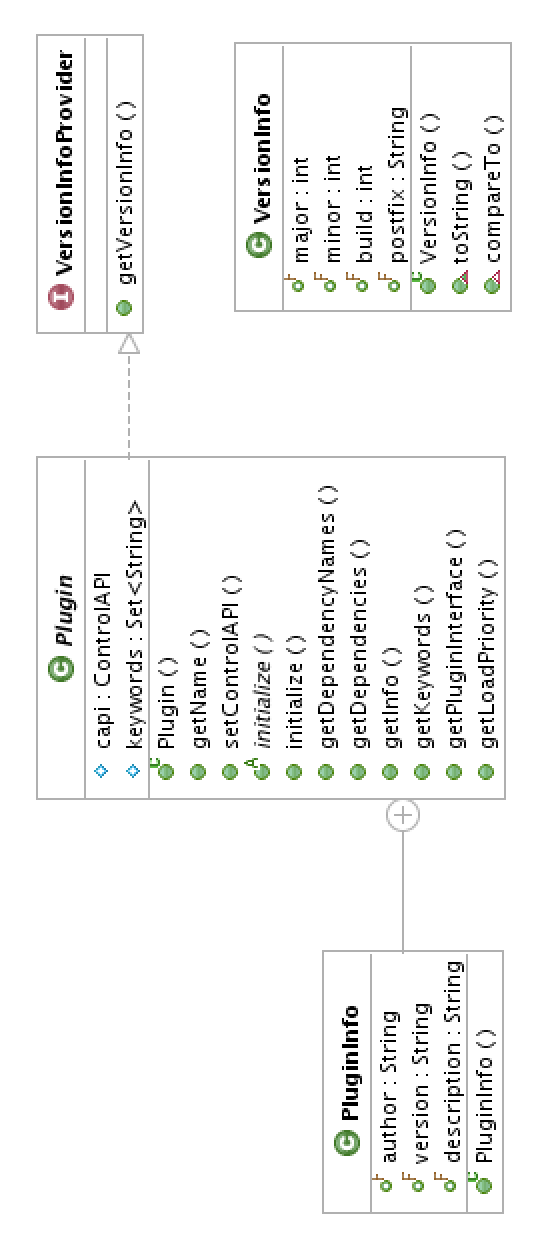
\includegraphics[angle=-90,width=\textwidth]{figures/PluginClass.eps}
\caption{CoreASM \code{Plugin} Abstract Class}
\label{fig:pluginClass}
\end{figure}
 
The \code{Plugin}\cindex{Plugin} class provides the core structure of \CoreASM plug-ins (see Figure~\ref{fig:pluginClass}). 
In its basic form, every \CoreASM plug-in should have a name, an initialize method, and a set of dependency requirements. 
%The \code{Plugin} class has the following methods:  
\begin{itemize}
	\item \code{getName()} returns the name of this Plug-in, which is the name of the runtime class of this plugin.

    \item The abstract method \code{initialize()} is called by the engine to initialize the plug-in. 
	\CoreASM plug-ins implement this method to perform custom initialization; e.g., registration 
    of operators in the engine.

	\item \code{getDependencyNames()} provides the names of the plugins that this plugin depends on. 
	It should return an empty set if there is no dependency requirement for this plugin. By default, 
	it returns an empty set.

	\item \code{getDependencies()} provides a map of {\em name} $\rightarrow$ {\em version-information} of the plugins 
	on which this plugin depends on. The version-information is the minimum version the required plugin should have. 
	This method should return an empty map if there is no dependency requirement for this plugin. By default, this method 
	will return the dependency names (see above) with a minimum version of `0.0.0'. 

	\item \code{getInfo()} returns some information about this plugin in an instance of \code{PluginInfo}\cindex{PluginInfo} object.

%     /**
%     * If this plugin implements the <code>ParserPlugin</code> 
%     * interface, this method extracts a set of keywords out 
%     * of grammar rules provided by this plugin.
%     * 
%     * @return a set of keywords (as Strings) 
%     */

	\item \CoreASM plug-ins can override \code{getPluginInterface()} to return an interface to provide custom services to engine's 
	environment (i.e., GUIs, tools, etc.). 

	\item \code{getLoadPriority()} returns the suggested loading priority of this plug-in. Zero is the lowest priority and 100 
	is the highest loading priority. The engine will consider this priority when loading plug-ins. All plug-ins with the same 
	priority value will be loaded in a non-deterministic order.  
 
\end{itemize}

\subsection{Our First Plug-in}

As we mentioned earlier, \CoreASM plug-ins are subclasses of the abstract class \code{Plugin}\cindex{Plugin}. 
As a result, every \CoreASM plug-in should at least implement the following two methods: \code{initialize()} and \code{getVersionInfo()}. 

To create our first plug-in, we create a Java class
\code{FirstSamplePlugin.java}\cindex{FirstSamplePlugin} (see
Program~\ref{pro:firstsample}) extending the \code{Plugin} class. In this
plug-in, we don't need to do anything for initialization, so we leave the
method empty. For version information, we create a new static instance of
\code{VersionInfo}\cindex{VersionInfo} and return it in the
\code{getVersionInfo()} method. 

\begin{program}
\small
\begin{verbatim}
package myplugins.firstplugin;

import org.coreasm.engine.VersionInfo;
import org.coreasm.engine.plugin.Plugin;

public class FirstSamplePlugin extends Plugin {

    public static final VersionInfo verInfo = new VersionInfo(0, 1, 1, "alpha");
	
    @Override
    public void initialize() {
        // do nothing
    }

    public VersionInfo getVersionInfo() {
        return verInfo;
    }

}
\end{verbatim}
\caption{\code{FirstSamplePlugin.java}}
\label{pro:firstsample}
\end{program}

As you can see, our first plug-in basically does nothing! We keep it simple for now and will later  
improve this plug-in to actually extend various aspects of the engine.

Before we continue, let's organize things a bit. We create a folder for our plugin, with two subfolders
\code{src} and \code{bin} to keep the source file and the binary file of plug-in. 
 
\begin{shell}
\begin{verbatim}
$ cd firstPlugin
$ ls
bin  src
$ tree
.
|-- bin
`-- src
    `-- myplugins
        `-- firstplugin
            `-- FirstSamplePlugin.java
$ _
\end{verbatim}
\end{shell}

\subsection{Deploying Our First Plugin}

Now that we created our plug-in class, we need to pack it properly so that the \CoreASM engine
can load it. This process has four steps:
\begin{enumerate}
	\item compiling the Java class(es)
	\item creating the plug-in id file; every \CoreASM plug-in needs to have an identification
		file that holds the absolute name of the plug-in class 
	\item packing the compiled class(es) together with the id file into a single JAR file
	\item copying the JAR file to the \CoreASM plugins folder 
\end{enumerate} 

\paragraph{Compiling} There are many ways to compile your Java class files. Here we simply call the 
Java compiler from the command line. To compile a plug-in, the binary class files of the \CoreASM engine
must be in your classpath. To make it short, we assume that these binary files are in `\code{../CoreASMBin}'.

\begin{shell}
\begin{verbatim}
$ javac -cp ../CoreASMBin:bin -sourcepath src -d bin src/myplugins/firstplugin/FirstSamplePlugin.java
$ tree 
.
|-- bin
|   `-- myplugins
|       `-- firstplugin
|           `-- FirstSamplePlugin.class
`-- src
    `-- myplugins
        `-- firstplugin
            `-- FirstSamplePlugin.java
$ _
\end{verbatim}
\end{shell}

\paragraph{Plug-in Id} To create the plug-in identification file use your favorite editor to 
create a plain text file named \code{CoreASMPlugin.id} with the following line:

\begin{center}\code{myplugins.firstplugin.FirstSamplePlugin}\end{center}

Move \code{CoreASMPlugin.id} file to the \code{bin} folder.

\paragraph{Packaging} Now that we have all the required files, we need to pack them together in 
a JAR file named `\code{FirstSamplePlugin.jar}'. The JAR file should contain the compiled Java 
classes (contents of the \code{bin} folder)
together with the identification file.    

\begin{shell}
\begin{verbatim}
$ cd bin
$ ls
CoreASMPlugin.id  myplugins
$ jar cf ../FirstSamplePlugin.jar CoreASMPlugin.id myplugins/
$ cd ..
$ ls
bin  FirstSamplePlugin.jar  src
$ _
\end{verbatim}
\end{shell}

\paragraph{Installing} The last step is to copy the JAR file to the `\code{plugins}' folder of 
the \CoreASM engine installed on your system. To check if everything is done properly, we can 
run \Carma with `\code{--version}' option to get a list of all the installed plug-ins:

\begin{shell}
\begin{verbatim}
$ carma --version
Carma 0.5.0-beta by Roozbeh Farahbod
CoreASM Engine 0.9.1-beta
Plugins: 
   PlotterPlugin 0.2.0-alpha
   NumberPlugin 0.5.0-beta
   ConditionalRulePlugin 0.9.0-beta
   FirstSamplePlugin 0.1.1-alpha              <----
   Kernel 0.7.1-beta
   TabBlocksPlugin 0.1.0-alpha
   BlockRulePlugin 0.9.0-beta
   ExtendRulePlugin 0.8.0-beta
   TurboASMPlugin 0.8.1-beta
   ChooseRulePlugin 0.9.0-beta
   ForallRulePlugin 0.9.0-beta
   StringPlugin 0.3.0-beta
   IOPlugin 0.3.0-beta
   PredicateLogicPlugin 0.4.1-beta
   LetRulePlugin 0.9.0-beta
   ListPlugin 0.2.0-alpha
\end{verbatim}
\end{shell}

Congratulations! In the following sections, we focus on improving the plug-in by implementing the interfaces listed in Table~\ref{tab:interfaces}.
We will not repeat the above procedure as it would be virtually the same.  

\section{Adding A New Function to \CoreASM}
\label{sec:newfunctions}

In this section, we will extend the abstract storage of the engine 
by adding a new function to the state.
To do so, we first look at the structure of a \CoreASM state.

\subsection{\CoreASM State Structure}

A \CoreASM state\index{CoreASM state@\CoreASM state} is composed of {\em
universes}\index{universe}, {\em functions}\index{function}, and {\em
rules}\index{rule}. Values in a \CoreASM state are represented by {\em
elements}\index{element}. Any value in the state is an instance of either the
root class \code{Element}\cindex{Element} or one of its subclasses. Universes,
functions, and rules are also elements. This would allow universes, functions,
and rules to be treated as values if needed.  Universes are defined by their
characterisitc function over elements of the states.

\begin{figure}
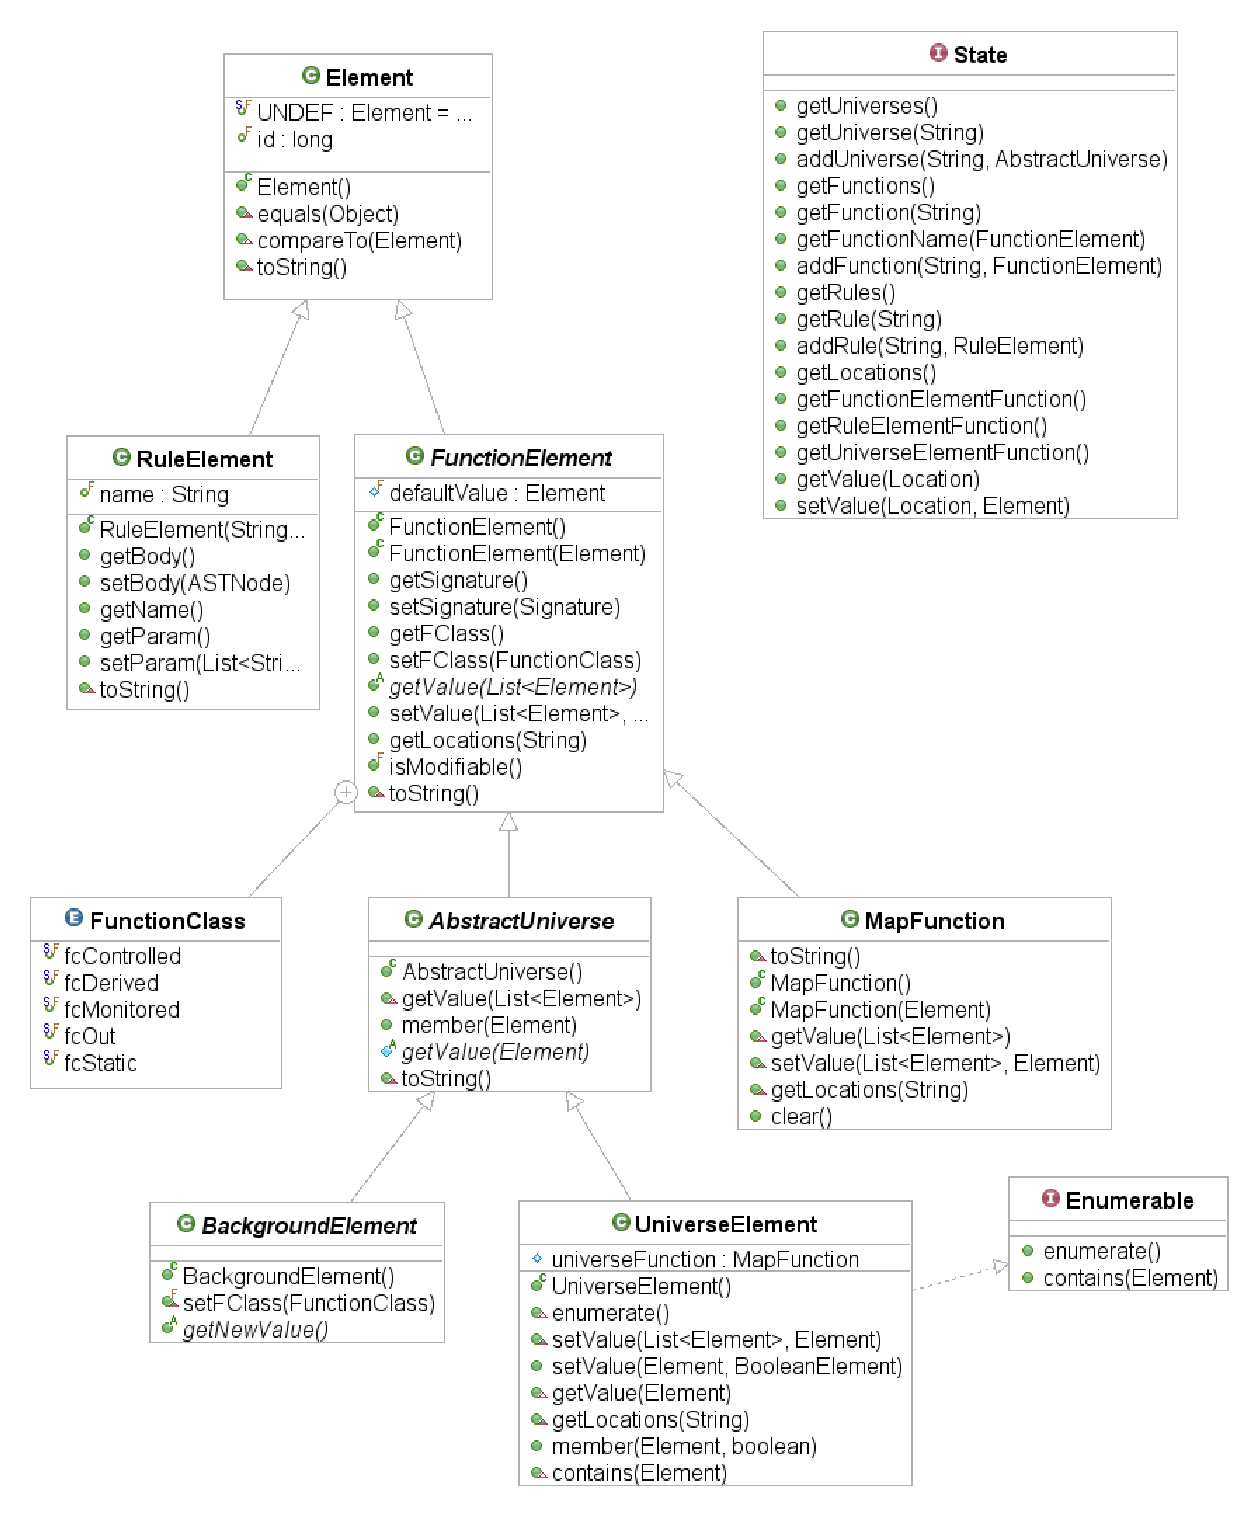
\includegraphics[width=\textwidth]{figures/AbstractStorageStructure.eps}
\caption{Elements, Rules, Functions, and Universes in Abstract Storage}
\label{fig:absstorage}
\end{figure}

Figure~\ref{fig:absstorage} presents a class diagram of the core classes and interfaces
contributing to the structure of a \CoreASM state.\footnote{Java package: \code{org.coreasm.engine.absstorage} }
The abstract class \code{FunctionElement}\cindex{FunctionElement} is the super
class of all function elements in the state.  Standard dynamic functions in ASM are
implemented by the \code{MapFunctionElement}\cindex{MapFunctionElement} class
which is an implementation of \code{FunctionElement} using maps.  Universes are
implemented by the \code{UniverseElement}\cindex{UniverseElement} class which
is itself a sublcass of \code{FunctionElement}. The
\code{BackgroundElement}\cindex{BackgroundElement} class implements backgrounds
as static universes.

The interface to a \CoreASM state is defined by the Java interface
\code{State}\cindex{State} (see Figure~\ref{fig:absstorage}).  Through this
interface, other components of the engine can add new functions, universes, and
rules or query about existence of those elements.  Plug-ins, as well as other
components of the engine, can also set and get values of locations of the state
using the \code{getValue} and \code{setValue} methods of this interface.
   
\subsection{Our Second Plug-in}

For our second plug-in, we extend the \CoreASM state by introducing a new derived function 
to calculate a hash value for String elements. We define the signature of this function
as:

\[ \Rfsig{hashValue}{String}{Number} \]

To provide the semantics of this function, we extend the \code{FunctionElement} class by 
a new class called \code{HashValueFunction} and we override the \code{getValue} of this 
class to calculate a hash value for the input String argument. See Program~\ref{pro:hashfunction}
for the actual implementation of this class. We will see later how our second plug-in instanciates 
this function and offers it to the engine to be added to the \CoreASM state.

\begin{program}
\small
%~~\begin{minipage}{0.95\textwidth}
%\begin{listing}[5]{1}
\begin{verbatim}
package myplugins.secondplugin;

import java.util.List;

import org.coreasm.engine.absstorage.Element;
import org.coreasm.engine.absstorage.FunctionElement;
import org.coreasm.engine.stdplugins.number.NumberElement;
import org.coreasm.engine.stdplugins.string.StringElement;

/** 
 * A CoreASM function to calculate a hash on String values
 */
public class HashValueFunction extends FunctionElement {

    @Override
    public Element getValue(List<Element> args) {
        Element result = Element.UNDEF;
        
        // if there is only one argument passed to this function
        if (args.size() == 1) { 
            Element argument = args.get(0);
            
            // if this argument is a StringElement
            if (argument instanceof StringElement) {
                result = new NumberElement(argument.toString().hashCode());
            }
            
        }
        
        return result;
    }

}
\end{verbatim}
%\end{listing}
%\end{minipage}
\caption{Hash Function Class}
\label{pro:hashfunction}
\end{program}

Our second plug-in is a bit more complicated than the first one. We are adding a new function that
takes a String element as input and provides a Number element as output. So, our plug-in depends on 
both the StringPlugin and the NumberPlugin. We should acknowledge this by overriding the \code{getDependencyNames()}
method of the \code{Plugin} class and instead of an empty set return a set consisting of ``StringPlugin'' 
and ``NumberPlugin'' as Java String objects (see Program~\ref{pro:secondplugin}).  

To tell the engine that this plug-in extends the \CoreASM state, we implement the \code{VocabularyExtender}\cindex{VocabularyExtender}
plug-in. This would require us to implement six more methods: \code{getFunctions()}, \code{getUniverses}, \code{getBackgrounds}, 
and similar ones for the names of these elements. We create a mapping of the String constant ``hashValue'' to an instance of 
our \code{HashFunctionElement} and return this map in the \code{getFunctions()} method. To keep a single instance of
this hash function, we use the \code{initialize} method to create and save an instance of this function.
That's all! The Java source code of our second plugin is presented in Program~\ref{pro:secondplugin}. 
We can now complile and deploy this plugin as we did for our first plugin.

With this new plug-in, the following \CoreASM specification would be valid:

\bExample
\codebf{CoreASM} TestSecondSamplePlugin\\
\\
\codebf{use} NumberPlugin\\
\codebf{use} StringPlugin\\
\codebf{use} SecondSamplePlugin\\
\codebf{use} IOPlugin\\
\\
\codebf{init} Main\\
\\
\codebf{rule} Main = \\
\tab \codebf{print} hashValue("R Farahbod")\\
\eExample

\noindent and running it with \Carma would result in the following (or similar) output:

\begin{shell}
\begin{verbatim}
$ carma -s 1 TestPlugin.coreasm
* Carma * : Loading the specification.
* Carma * : Performing the initial step.
4.9477543E7
* Carma * : Starting the execution.

4.9477543E7

* Carma * : Stopped after 1 steps.
* Carma * : Execution concluded.
$ _
\end{verbatim}
\end{shell}


\begin{program}
\small
\begin{verbatim}
package myplugins.secondplugin;

import org.coreasm.engine.VersionInfo;
import org.coreasm.engine.plugin.Plugin;
import org.coreasm.engine.plugin.VocabularyExtender;
import org.coreasm.engine.absstorage.*;
import java.util.*;

public class SecondSamplePlugin extends Plugin implements VocabularyExtender {

    public static final VersionInfo verInfo = new VersionInfo(0, 2, 1, "alpha");
    private Map<String,FunctionElement> functions = null;
    private FunctionElement hashValueFunction;
    private final Set<String> dependencySet;

    public SecondSamplePlugin() {
        super();
        dependencySet = new HashSet<String>();
        dependencySet.add("StringPlugin");
        dependencySet.add("NumberPlugin");
    }

    @Override
    public void initialize() { hashValueFunction = new HashValueFunction(); }

    public VersionInfo getVersionInfo() { return verInfo; }

    @Override
    public Set<String> getDependencyNames() { return this.dependencySet; }
	
    public Map<String,FunctionElement> getFunctions() {
        if (functions == null) {
            functions = new HashMap<String,FunctionElement>();
            functions.put("hashValue", hashValueFunction);
        }
        return functions;
    }

    public Set<String> getFunctionNames() { return functions.keySet(); }

    public Map<String,UniverseElement> getUniverses() { return Collections.emptyMap(); }

    public Set<String> getUniverseNames() { return Collections.emptySet(); }

    public Set<String> getBackgroundNames() { return Collections.emptySet(); }

    public Map<String,BackgroundElement> getBackgrounds() { return Collections.emptyMap(); }
}
\end{verbatim}
\caption{\code{SecondSamplePlugin.java}}
\label{pro:secondplugin}
\end{program}

%\section{Adding a New Rule}
%\label{sec:newrule}

%\medskip \noindent
%{\bf Acknowledgments.} We would like to thank Mashaal Memon for his
%contribution to the \CoreASM project and for many constructive discussions regarding
%the plug-in architecture. Our sincere appreciation to Egon B{\"o}rger for 
%persistent encouragement and valuable feedback on the \CoreASM project. 

\printindex

\end{document}

